%
% A (non-exhaustive) list of TODOs:
%
% - write appendix displaying adiabatic elimination of a lossy mode for an arbitrary operator. 

\chapter{PhoG: Photon Gun}\label{chapter:phog}
Goal of chapter: analyse and model the PhoG device and its efficacy for producing, from a classical input, (i) bright sub-Poissonian state; (ii) entangled state


\section{Introduction}
\begin{itemize}
\item Introduce dissipation as a means for state engineering
\item Introduce our goal to produce single-photons (or close to single-photons)
\item Introduce this chapter, include a chapter outline, and provide motivation for why we will look at different models
\end{itemize}

\begin{figure}[htp]
\centering
\includegraphics[draft=false, width=\linewidth]{phog/phog_models}
\caption{\label{fig:phog_models} Hierarchy of models of the phog device, from least realistic (left) to most realistic (right). We will discuss each model in turn throughout the rest of this chapter. \MakeUppercase{\romannumeral 1}: Single-mode model. \MakeUppercase{\romannumeral 2}: Two-mode model. \MakeUppercase{\romannumeral 3}: Three-mode model. \MakeUppercase{\romannumeral 4}: Multi-mode model. \MakeUppercase{\romannumeral 5} Multi-mode model embedded in glass. }
\end{figure}

\section{Single-mode model}\label{sec:phog_single_mode_model}

\begin{figure}[htp]
\centering
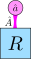
\includegraphics[width=0.2\linewidth, draft=false]{phog/single_mode}
\caption{\label{fig:phog_single_mode} A single bosonic mode, $a$, is coupled to a Markovian reservoir $R$ by operator $\hat{A}$. }
\end{figure}

\MT{Make sure that my analysis in this section is sufficiently motivated and doesn't seem like too much of a detour.}

Consider the model displayed in Fig.~\ref{fig:phog_single_mode} (c.f. Fig.~\ref{fig:phog_models}\MakeUppercase{\romannumeral 1}), which consists of a single bosonic mode, $a$, coupled to a reservoir $R$ via a reservoir operator $\mathcal{A}$. The annihilation (creation) operator for mode $a$ is denoted $\hat{a} \left(\hat{a}^\dagger\right)$, and the density matrix containing all information about the state of the mode is denoted $\rho_a$. This model will prove illustrative of several principles which we will develop throughout the chapter. Assuming that reservoir $R$ is Markovian, the evolution of mode $a$ is given by the following quantum master equation in Lindblad form\footnote{Equations in this form will be referred to as ``Lindblad equations''}

\begin{equation}\label{eqn:phog_lindblad_1}
\ddt \rho_a =  - i \left[\hat{H}, \rho_a\right] + \gamma \mathcal{L}\left(\hat{A}\right)\rho_a
\end{equation}

\noindent In what follows we consider the case with Hamiltonian $\hat{H} = \hbar \omega \hat{a}^\dagger \hat{a}$. Eq.~\ref{eqn:phog_lindblad_1} then describes the decay of state $\rho_a\left(t=0\right)$ into $R$ with rate $\gamma$. The Lindbladian term $\mathcal{L}\left(\hat{A}\right)$ takes the usual form
\begin{equation}\label{eqn:phog_lindbladian_form}
\mathcal{L}\left(\hat{A}\right)\rho_a = \hat{A}\rho_a\hat{A}^\dagger - \frac{1}{2} \hat{A}^\dagger \hat{A} \rho_a - \frac{1}{2} \rho_a \hat{A}^\dagger \hat{A}.
\end{equation}

\noindent Let us consider the behaviour of an initially coherent state $\rho_a\left(t=0\right) = \dyad{\alpha}$ with amplitude $\alpha$. We will explore several choices for decay operator $\hat{A}$.

\subsection{$\hat{A} = \hat{a}$}
First, we will explore the case where the decay into the reservoir is governed by mode $a$ annihilation operator, $\hat{a}$, which corresponds to single-photon loss.% I can refer to intro chapter for properties of this.
The evolution of $\rho_a$ is described by

\begin{equation}\label{eqn:phog_lindblad_single_photon_loss}
\ddt \rho_a = \gamma\left[\hat{a}\rho_a \hat{a}^\dagger - \frac{1}{2} \hat{a}^\dagger \hat{a} \rho_a - \frac{1}{2} \rho_a \hat{a}^\dagger \hat{a}\right],
\end{equation}
where we have transformed into a rotating frame and so the free Hamiltonian term $\hbar \omega \hat{a}^\dagger \hat{a}$ vanishes. Let us calculate the evolution $\langle \hat{a}^\dagger \hat{a}\rangle\left(t\right)$ of photon number expectation:

\begin{align}
\ddt \langle \hat{a}^\dagger \hat{a}\rangle &= \gamma \left[ \text{Tr}\left(\hat{a}^\dagger \hat{a} \hat{a} \rho_a \hat{a}^\dagger \right) - \frac{1}{2} \text{Tr}\left(\hat{a}^\dagger \hat{a} \hat{a}^\dagger \hat{a} \rho_a\right) - \frac{1}{2} \text{Tr}\left(\hat{a}^\dagger \hat{a} \rho_a \hat{a}^\dagger \hat{a}\right)\right] \notag \\
%
&= \gamma \left[ \langle \hat{a}^\dagger \hat{a}^\dagger \hat{a}\hat{a}\rangle - \langle \hat{a}^\dagger \hat{a} \hat{a}^\dagger \hat{a}\rangle \right] \notag \\
%
&= - \gamma \langle \hat{a}^\dagger \hat{a}\rangle
\end{align}
\noindent and so
\begin{equation}\label{eqn:phog_single_photon_loss_number_expectation}
\langle\hat{a}^\dagger \hat{a} \rangle \left(t\right) = \langle \hat{a}^\dagger \hat{a}\rangle \left(0\right) e^{- \gamma t}
\end{equation}
the photon number exponentially decays in time with decay rate $\gamma$. We may derive similar equations for $\langle\hat{x}\rangle\left(t\right)$ and $\langle\hat{x}\rangle\left(t\right)$ and find 
\begin{align}\label{eqn:phog_single_photon_loss_quadrature_expectation}
 \langle \hat{x}\rangle\left(t\right) &= \langle \hat{x}\rangle\left(0\right) e^{- \frac{\gamma}{2} t} \notag \\
%
 \langle \hat{p}\rangle\left(t\right) &= \langle \hat{p}\rangle \left(0\right) e^{- \frac{\gamma}{2} t}.
\end{align}

\noindent We might guess that the steady-state of Eq.~\ref{eqn:phog_lindblad_single_photon_loss} is the vacuum $\dyad{0}$, and indeed we can deduce that this must be the case by noticing that $\ddt \rho_a = 0$ when $\rho_a$ is vacuum. In Fig.~\ref{fig:phog_lindblad_single_photon_loss}a we plot the evolution of $\langle\hat{a}^\dagger \hat{a}\rangle, \langle \hat{x}\rangle, \langle \hat{p}\rangle$ and see that the photon number expectation and quadrature expectations decay towards zero, confirming Eqs.~\ref{eqn:phog_single_photon_loss_number_expectation},~\ref{eqn:phog_single_photon_loss_quadrature_expectation}, while the variances in $\hat{x}$ and $\hat{p}$ remain constant. This might lead us to conclude that the state $\rho_a\left(t\right)$ remains a coherent state with decreasing amplitude $\alpha\rightarrow0$, until it reaches the vacuum state.

In Fig.~\ref{fig:phog_lindblad_single_photon_loss}b we plot the fidelities $\mathcal{F}$ between $\rho_a\left(t\right)$ and the vacuum state $\dyad{0}$, the single-photon state $\dyad{1}$ and a coherent state $\dyad{\alpha^\prime}$ with $\left|\alpha^\prime\right|^2 = \langle \hat{n}\rangle_{\rho_a}\left(t\right)$, in other words the coherent state with same photon-number expectation as $\rho_a$. We observe that the fidelity to the vacuum state increases to $1$ while the fidelity to coherent state $\dyad{\alpha^\prime}=1$ always, which confirms our intuitions that $\rho_a$ remains coherent $\forall t$ and that $\dyad{0}$ is the steady state.


\begin{figure}[htp]
\centering
	\begin{subfigure}{0.6\linewidth}
	\centering
	\includegraphics[draft=false, width=\linewidth]{phog/expects_a}
	\caption{}
	\end{subfigure}
	\begin{subfigure}{0.6\linewidth}
	\centering
	\includegraphics[draft=false, width=\linewidth]{phog/fidelities_a}
	\caption{}
	\end{subfigure}
\caption{\label{fig:phog_lindblad_single_photon_loss}$\hat{A} = \hat{a}$. (a) Operator expectation values calculated for state $\rho_a\left(t\right)$ as it evolves under Eq.~\ref{eqn:phog_lindblad_single_photon_loss}. An initial coherent state $\alpha=3.0$ decays to vacuum state $\dyad{0}$. Quadrature variances remain constant through time, implying that $\rho_a$ remains a coherent state throughout its evolution. This is confirmed in (b) where the fidelity between $\rho_a$ and $\dyad{\alpha^\prime}$ is demonstrated to remain $1$ for all time. The amplitude $\alpha^\prime$ is chosen to give a coherent state with equivalent photon-number expectation to $\rho_a\left(t\right)$. Horizontal gridlines displayed in black, dashed.}
\end{figure}

\subsection{$\hat{A} = \hat{a}^2$}
Next we consider a two-photon loss term $\hat{a}^2$, which describes two-photon decay into the reservoir. Our Lindblad equation is

\begin{equation}\label{eqn:phog_lindblad_two_photon_loss}
\ddt \rho_a = \gamma\left[\hat{a}^2 \rho_a \hat{a}^{\dagger 2} - \frac{1}{2} \hat{a}^{\dagger 2} \hat{a}^2 \rho_a - \frac{1}{2} \rho \hat{a}^{\dagger 2} \hat{a}^2\right]
\end{equation}
which gives the evolution of photon number expectation as 
\begin{equation}
\ddt \langle \hat{a}^\dagger \hat{a}\rangle = - 2 \gamma \langle \hat{a}^\dagger \hat{a}^\dagger \hat{a}\hat{a}\rangle
\end{equation}
which does not take a closed form and so we cannot yet directly calculate $\langle \hat{a}^\dagger \hat{a}\rangle\left(t\right)$. Similarly, equations for evolution of $\langle\hat{a}\rangle\left(t\right)$ require terms to the third power in the creation/annihilation operators, and so are not yet closed.  We will see techniques in Sec.~\ref{sec:linearization} which allow us to deal with this.

\MT{TODO: expand this discussion to allow for mixedness in output state.}
For now, let us deduce what must be the steady-state of Eq.~\ref{eqn:phog_lindblad_two_photon_loss}. We observe that once again the vacuum $\dyad{0}$ must be a steady state, since then $\ddt \rho_a=0$. Surprisingly we now also have the single-photon state $\dyad{1}$ as a steady state since this also has $\ddt \rho_a=0$. The general steady-state is a superposition of these
\begin{equation}\label{eqn:phog_phase_state}
\ket{\psi} = \ket{0} + e^{i \phi} \ket{1} \qq{with} \rho_a\left(t \rightarrow \infty\right) = \dyad{\psi}
\end{equation}
which takes the form of a so-called \emph{phase state}, and has long been known that the steady state of two-photon loss is a phase-state. The phase $\phi$ is related to the phase of the initial coherent state. %\MT{show this.}


In Fig.~\ref{fig:phog_lindblad_two_photon_loss}a we plot the evolution of $\langle \hat{a}^\dagger \hat{a}\rangle, \langle \hat{x}\rangle, \langle \hat{p}\rangle$ and the quadrature variances. The photon number expectation no longer decays to zero as it did for $\hat{A}=\hat{a}$. In Fig.~\ref{fig:phog_lindblad_two_photon_loss}b we observe the fidelity between $\rho_a\left(t\right)$ and the final phase state increases to $\MT{X}$, and so we see that two-photon loss induces nonclassicality in the system. \MT{I should talk about the mixedness of the state somewhere.}


\begin{figure}[htp]
\centering
	\begin{subfigure}{0.6\linewidth}
	\centering
	\includegraphics[draft=false, width=\linewidth]{phog/expects_aa}
	\caption{}
	\end{subfigure}
	\begin{subfigure}{0.6\linewidth}
	\centering
	\includegraphics[draft=false, width=\linewidth]{phog/fidelities_aa}
	\caption{}
	\end{subfigure}
\caption{\label{fig:phog_lindblad_two_photon_loss}$\hat{A} = \hat{a}^2$. (a) Operator expectation values for state $\rho_a\left(t\right)$ as it evolves under Eq.~\ref{eqn:phog_lindblad_two_photon_loss}. An intially coherent state with $\alpha=3.0$ no longer decays to the vacuum state, and the final photon-number expectation is nonzero. The quadrature variances are no longer constant which implies that the state is no longer coherent, which is confirmed in (b) where the fidelity between $\rho_a\left(t\right)$ and $\dyad{\alpha^\prime}$ is plotted. The fidelity between $\rho_a\left(t\right)$ and steady state increases to \MT{X}. Horizontal gridlines displayed in black, dashed.}
\end{figure}



\subsection{$\hat{A} = \hat{a}^3$}
We might guess that the steady state $\ket{\psi}$ of the three-photon loss term $\hat{a}^3$ is likewise a superposition of $\ket{0}, \ket{1}$ and $\ket{2}$
\begin{equation}\label{eqn:phog_three_photon_loss_ss}
\rho_a\left(t\rightarrow\infty\right) = \frac{\dyad{\psi}}{3} \qq{with} \ket{\psi} \stackrel{?}{=} \ket{0} + e^{i \phi}\ket{1} + e^{i \varphi}\ket{2}
\end{equation}
\MT{check how the state is normalized}
with phases $\phi, \varphi$ in general depending on the initial coherent state $\dyad{\alpha}$. %\MT{TODO: investigate this numerically}.
Indeed, we can deduce that Eq.~\ref{eqn:phog_three_photon_loss_ss} must be a steady state of the system by noting that $\hat{a}^3 \ket{\psi} = 0$ which implies $\ddt \rho_a = 0$.

%\MT{TODO: analytically show in fock basis the steady state}

We plot the evolution of fidelities between $\rho_a\left(t\right)$ evolving with decay operator $\hat{a}^3$ in Fig.~\ref{fig:phog_lindblad_three_photon_loss}. We see the fidelity to the state in Eq.~\ref{eqn:phog_three_photon_loss_ss} increasing to \MT{X}. \MT{additional comments.}

\begin{figure}[htp]
\centering
\includegraphics[draft=false, width=0.6\linewidth]{phog/fidelities_aaa}
\caption{\label{fig:phog_lindblad_three_photon_loss}$\hat{A} = \hat{a}^3$ (a) Fidelities between state $\rho_a\left(t\right)$ and vacuum (red), single-photon state (orange), coherent state with equivalent photon-number expectation to $\rho_a$ (green), and the two-phase state (blue). \MT{additional comments/interpretation.} Horizontal gridlines displayed in black, dashed.}
\end{figure}

\clearpage
\subsection{$\hat{A} = \hat{a}\left(\hat{a}^\dagger \hat{a} - 1\right)$}\label{sec:phog_single_mode_ncl_1}
We have seen that the choice of $\hat{A}$ can give drastically different steady states of $\rho_a$,  from the uninteresting vacuum to the highly quantum and useful phase-state. We therefore wish to consider which choices for $\hat{A}$ will give rise to a Fock state $\dyad{n}$

The choice 
\begin{equation}\label{eqn:phog_A_ncl}
\hat{A} = \hat{a}\left(\hat{a}^\dagger \hat{a} - 1\right)
\end{equation}
may be interpreted as a single-photon loss with a rate which depends on photon number. We can see that the loss rate will go to zero for state $\dyad{1}$, and so suspect that the single-photon state $\dyad{1}$ is a steady state of this loss mechanism.

The Lindblad equation which we solve is
\begin{equation}\label{eqn:phog_ncl_lindblad}
\ddt \rho_a = \gamma \left[ \hat{a}\left(\hat{n}-1\right) \rho \left(\hat{n}-1\right)\hat{a}^\dagger - \frac{1}{2} \rho \left(\hat{n}-1\right) \hat{n} \left(\hat{n}-1\right) - \frac{1}{2} \left(\hat{n}-1\right)\hat{n}\left(\hat{n}-1\right) \rho \right]
\end{equation}
and for convenience we have written the photon-number operator $\hat{n}$ where possible.
%The vacuum state $\dyad{0}$ also happens to be a steady-state of $\ncl$, but \MT{its coefficient remains constant, so we obtain $\dyad{1}$ in the limit of $\alpha\rightarrow \infty$}
We examine the evolution of $\rho_a$ in Fig.~\ref{fig:phog_A_ncl} and plot the evolution of photon number, $\langle \hat{x}\rangle, \langle \hat{p}\rangle$ in (a). We observe non-exponential decay of photon-number expectation to $1$ %TODO: show that it is non-exponential. (e.g. try fitting an exponential to it)
while in (b) the fidelity between $\rho_a\left(t\right)$ and $\dyad{1}$ increases to $1$, implying that this choise of $\hat{A}$ does indeed have a single-photon steady state. Even after short times $t < 0.1$ the fidelity to an equivalent coherent state quickly decreases (and the quadrature variances quickly increase over similar timescale), implying a rapid increase in non-classicality of the system.\footnote{We shall explore and quantify this later.}

Therefore, we deduce that the decay operator $\hat{a}\left(\hat{a}^\dagger \hat{a} - 1\right)$ is a useful candidate for driving our system towards the highly nonclassical single-photon state. In the remainder of this chapter our goal will be to find a physical system which can efficiently implement this decay operator.



\begin{figure}[htp]
\centering
	\begin{subfigure}{0.6\linewidth}
	\centering
	\includegraphics[width=\linewidth, draft=false]{phog/expects_ncl1}
	\caption{}
	\end{subfigure}
	\begin{subfigure}{0.6\linewidth}
	\centering
	\includegraphics[width=\linewidth, draft=false]{phog/fidelities_ncl1}
	\caption{}
	\end{subfigure}
\caption{\label{fig:phog_A_ncl}$\hat{A} = \hat{a}\left(\hat{a}^\dagger \hat{a} - 1\right)$ (a) Operator expectation values for state $\rho_a\left(t\right)$ as it evolves. An initially coherent state with $\alpha=3.0$ decays to a state with $\langle \hat{n}\rangle=1$, which we confirm as state $\dyad{1}$ by considering the fidelity in (b). Horizontal gridlines displayed in black, dashed.}
\end{figure}

To gain some insight into the action of $\ncl$ let us first write the Lindblad equation~\ref{eqn:phog_ncl_lindblad} in Fock basis for density matrix element $\rho_{m, n}$
\begin{align}\label{eqn:phog_ncl_lindblad_fock}
&\ddt \rho_{m, n} = \bra{m} \ddt \rho \ket{n} \notag  \\
%
&= \gamma \left[ m \sqrt{m+1} n \sqrt{n+1} \, \rho_{m+1, n+1} - \frac{1}{2} \left(n-1\right)^2 n\, \rho_{m, n} - \frac{1}{2} \left(m-1\right)^2 m\, \rho_{m, n}\right],
\end{align}
and consider some specific matrix elements. Immediately we see that Eq.~\ref{eqn:phog_ncl_lindblad_fock} couples diagonal elements $m=n$ to diagonal elements and so an analysis of the photon-number statistics is possible only considering diagonal elements of the density matrix, and ignoring coherences. We obtain, for example $\ddt \rho_{1, 1}=2 \gamma \rho_{2, 2}$ which is greater than zero, and so $\forall t$ we expect the single-photon contribution $\rho_{1,1}$ to increase, c.f. Fig.~\ref{fig:phog_A_ncl}b. 

The elements $\rho_{0, 0}, \rho_{0, 1}$ and $\rho_{1, 0}$ give
\begin{equation}
\ddt \rho_{0,0} = 0, \qq{} \ddt \rho_{0, 1} = 0, \qq{and} \ddt\rho_{1, 0} = 0 
\end{equation}
which implies that these elements are constant in time. The single-photon state requires zero in each of these elements, and so we may predict that high fidelity between $\rho_a$ and $\dyad{1}$ may only be obtained when $\rho_{0,0}\left(t=0\right), \rho_{0, 1}\left(t=0\right), \rho_{1, 0}\left(t=0\right) \ll 1$. This implies, in particular, that high fidelity with $\dyad{1}$ is not obtainable for coherent states with small amplitude $\alpha$.\footnote{The requirement of large $\alpha$ for the input coherent state is not very restrictive, and as we shall see in the next section there are additional reasons to prefer $\alpha \gg 1$}. In Fig.~\ref{fig:phog_fidelity_ncl_vs_alpha} we show this explicitly.

\begin{figure}[htp]
\centering
\includegraphics[width=0.6\linewidth, draft=false]{phog/fidelities_ncl1_vs_alpha}
\caption{\label{fig:phog_fidelity_ncl_vs_alpha} The fidelity of $\rho_a\left(t\rightarrow\infty\right)$ to single-photon state $\dyad{1}$ depends on $\alpha$ since the density matrix elements $\rho_{0, 0}, \rho_{0, 1}$ and $\rho_{1, 0}$ are constant in time. This helps to quantify the intuition that in our lossy system a state with on average less than $1$ photon cannot be used to increase the photon number.}
\end{figure}




Before we move on, let us quickly explore the related operator $\hat{a}\left(\hat{a}^\dagger \hat{a} -2\right)$. Based on the above discussion we might reasonably expect the steady-state to be $\dyad{2}$, and this is indeed what we see in Fig.~\ref{fig:phog_A_ncl2}, where the fidelity to the two-photon state increases to $1$.

\begin{figure}[htp]
\centering
\includegraphics[width=0.6\linewidth, draft=false]{phog/fidelities_ncl2}
\caption{\label{fig:phog_A_ncl2} $\hat{A} = \hat{a}\left(\hat{a}^\dagger \hat{a} - 2\right)$. The steady-state of this loss operator is $\dyad{2}$ the fidelity of $\rho_a$ to this state increases to $1$.}
\end{figure}

\MT{add some references and chat about ``nonlinear coherent states''.}


\clearpage
\section{Including loss}\label{sec:phog_including_loss}
We have seen that the loss operator $\ncl$ is a good canditate for driving an initial coherent state towards a single photon state $\ket{1}$. Any system, therefore, which can implement the Lindblad equation~\ref{eqn:phog_lindblad_1} with $\hat{A} = \ncl$ will asymptotically give rise to single-photon Fock states, although fidelities close to $1$ are obtainable even at finite time, Fig.~\ref{fig:phog_A_ncl}b. 

In a realistic situation however it is unlikely that a system can be designed to implement $\ncl$ only, and so we must consider how the final states are affected by additional loss mechanisms. In an optical system the single-photon (``linear'') loss can never be avoided, so we will explore its effect on the nonlinear coherent loss mechanism. \MT{make sure I have defined NCL before now.} To do this, we modify our original Lindblad equation to
\begin{equation}\label{eqn:phog_lindblad_a_ncl}
\ddt \rho_a =  - i \left[ \hat{H}, \rho_a\right] + \gamma_1 \mathcal{L}\left(\hat{a}\right)\rho_a + \gncl \mathcal{L}\left(\ncl\right)\rho_a
\end{equation}
with $\gamma_1$ the decay rate via the single-photon loss channel $\hat{a}$, and $\gncl$ the loss rate via NCL $\ncl$.

We can immediately see that $\dyad{1}$ is only a steady-state of Eq.~\ref{eqn:phog_lindblad_a_ncl} when $\gamma_1 = 0$, in which case we revert to the analysis of Sec.~\ref{sec:phog_single_mode_ncl_1}. For all $\gamma_1 > 0$, $\dyad{0}$ is a steady-state, and a consideration of $\rho_{m, n}$ shows that $\rho_{0, 0}, \rho_{0, 1}, \rho_{1, 0}$ are no longer constant in time. 

Physically we see therefore that the presence of linear loss ($\gamma_1 > 0$) leads to a degradation of the highly-quantum output state which can be reached under NCL, as the single-photon loss mechanism pushes $\rho_a$ towards the vacuum. We see this explicitly in Fig.~\ref{fig:phog_A_ncl_loss}b (c.f. Fig.~\ref{fig:phog_A_ncl}), where an intially increasing fidelity with $\dyad{1}$ eventually dies away, and fidelity to the vacuum state increases to $1$. 

We examine the maximum attainable fidelity to $\dyad{1}$ in Fig.~\ref{fig:phog_max_fidelity}. The maximum fidelity decreases with increasing $\gamma_1$, but increasing $\alpha$ appears to allow larger fidelities to be reached at the same $\gamma_1$ (c.f. Fig.~\ref{fig:phog_fidelity_ncl_vs_alpha}). We will explore this phenomenon further in Sec.~\MT{X}.




\begin{figure}[htp]
\centering
	\begin{subfigure}{0.6\linewidth}
	\centering
	\includegraphics[width=\linewidth, draft=false]{phog/expects_ncl1_and_a}
	\caption{}
	\end{subfigure}
	\begin{subfigure}{0.6\linewidth}
	\centering
	\includegraphics[width=\linewidth, draft=false]{phog/fidelities_ncl1_and_a}
	\caption{}
	\end{subfigure}
\caption{\label{fig:phog_A_ncl_loss} NCL $\ncl$ and linear loss $\hat{a}$. Initial coherent state amplitude $\alpha=3.0$, and $\gncl=8.0$. (a) Operator expectation values. Solid: $\langle \hat{a}^\dagger \hat{a}\rangle$. The presence of linear loss $\gamma_1 > 0$ ensures that the photon number decays to $0$. Dashed: $\text{Var}\left(\hat{x}\right)$. Similarly, for $\gamma_1 > 0$ we see the variance in $x$ return to its initial value, hinting that our state is being pushed towards vacuum. (b) Fidelities of $\rho_a\left(t\right)$ against vacuum (blue), single-photon state (red) and coherent state with equivalent photon-number expectation (orange). Solid: $\gamma_1 = 0$. Dot-dashed: $\gamma_1 = 2$. Dashed: $\gamma_1 = 20$. The presence of linear loss pushes $\rho_a$ away from the single-photon state for $t > 0.1$. For $t < 0.1$ the system is dominated by NCL}
\end{figure}

%It is only for $t > 0.1$ that the fidelity decays, even for large $\gamma_1 = 20$, and for $t < 0.1$ the system seems dominated by NCL $\ncl$. 

\begin{figure}[htp]
\centering
\includegraphics[width=0.6\linewidth, draft=false]{phog/max_fidelities_vs_gamma1_ncl1_and_a}
\caption{\label{fig:phog_max_fidelity} Maximum attainable fidelity between $\rho_a$ and $\dyad{1}$ at different linear loss levels $\gamma_1$. Linear loss drives $\rho_a$ towards the vacuum and destroys the quantumness of our state, but over short times the fidelity to $\dyad{1}$ appears independent of $\gamma_1$, Fig.~\ref{fig:phog_A_ncl_loss}. Here, we observe that after $\gamma_1 \approx 7.5$ the maximum attainable fidelity is practically independent of linear loss rate, while it depends on $\alpha$. We shall explore this further in Sec.~\MT{X}.}
\end{figure}

Figure~\ref{fig:phog_A_ncl_loss}b suggests an interesting phenomenon: over short timescales the system appears to be dominated by NCL $\ncl$. Consider for example the fidelity between $\rho_a\left(t < 0.05\right)$ and $\dyad{\alpha^\prime}$ denoting a coherent state with equivalent photon-number expectation. By considering this alone, for short times the behaviour is indistinguishable from the case with $\gamma_1 = 0$. Similar reasoning applies also to the fidelities between $\rho_a\left(t < 0.1\right)$ and $\dyad{1}$, where the evolution is almost independent of $\gamma_1$.

From fidelity $\mathcal{F}\left( \rho_a\left(t<0.1\right), \dyad{0}\right)$, Fig.~\ref{fig:phog_A_ncl_loss} even suggests that $\gamma_1 \gg 0$ might help drive $\rho_a$ towards the single-photon state faster than in the lossless case. However we infer that loss actually is not helpful here, since after about $t=0.05$ the fidelity to $\dyad{\alpha^\prime}$ begins to increase again. This suggests that fidelity might not always be a useful measure of the desired behaviour when both nonlinear dissipation and linear loss are included.\footnote{Of course, we could have guessed this based on Fig.~\ref{fig:phog_lindblad_single_photon_loss}b as the fidelity to $\dyad{1}$ increases until $t\approx 0.25$ while the state remains completely coherent.}



\MT{ segue into talking about our two options. 1) reduce time evolution of our system. 2) use bright input state }

\subsection{Mandel parameter $Q$}
Although the fidelity is a helpful measure for measuring the ability of our system to produce single-photons, we have observed the case where fidelity to the single-photon increases while $\rho_a$ remains entirely coherent. It is therefore worth considering which other measures we might use to measure progress. One such measure is the Mandel $Q$ parameter \MT{cite}
\begin{equation}\label{eqn:phog_mandelQ}
Q = \frac{\ev{\Delta\hat{n}^2}}{\ev{\hat{n}}} - 1
\end{equation}
in terms of photon-number expectation $\ev{\hat{n}}$ and variance $\ev{\Delta\hat{n}^2}$. Eq.~\ref{eqn:phog_mandelQ} may equivalently be written as 
\begin{equation}
Q = \frac{\ev{\hat{a}^\dagger \hat{a}^\dagger \hat{a}\hat{a}}}{\ev{\hat{a}^\dagger \hat{a}}} - \ev{\hat{a}^\dagger \hat{a}}.
\end{equation}
Intuitively, Eq.~\ref{eqn:phog_mandelQ} is a measure of the level of photon-number squeezing in $\rho_a$. In the limit of zero uncertainty in photon-number, $\ev{\Delta\hat{n}} \rightarrow 0$ and so $Q \rightarrow -1$, while for a coherent state obeying Poissonian photon-number statistics $Q = 1$. We will therefore seek to find parameter regimes for which loss operators $\ncl$ or $\hat{a}^2$ give $Q<0$. 

%Using $Q$ as our measure to optimise has the advantage that it takes value $Q = -1$ for any Fock state and so knowledge of the steady-state of the system is not required. Additionally we do not require access to the full density matrix $\rho_a$ in order to calculate $Q$, and since $Q$ may be written entirely in terms of photon-number operator $\hat{n}$ we note that only the diagonal elements $\rho_{n, n}$ of $\rho_a$ are required. And as we observed in Sec.~\ref{sec:phog_single_mode_ncl_1}, the Lindblad equation~\ref{eqn:phog_A_ncl} couples diagonal elements to diagonal elements, which will allow for our analysis to be simplified.  \MT{Not sure where to put this paragraph or these statements.}

The effect of NCL $\ncl$ on $Q$ is displayed in Fig.~\ref{fig:phog_ncl_Q}a under several different linear loss rates $\gamma_1$. We see that the effect of NCL is indeed to drive $\rho_a$ towards a Fock state, and $Q \rightarrow -1$ for $\gamma_1 = 0$. For all $\gamma_1 \ne 0$ however we see that $Q$ eventually returns to $0$ as the system becomes vacuum. However, large $\left|Q\right|$ are obtained for finite $t$. In Fig.~\ref{fig:phog_ncl_Q} we observe that the behaviour of $Q$ is indeed identical over the initial evolution of $\rho_a$ and is independent of linear loss rate $\gamma_1$ which bodes well for implementation of $\ncl$ as a deterministic generator of single-photon states. 

\begin{figure}[htp]
\centering
	\begin{subfigure}{0.6\linewidth}
	\caption{}
	\includegraphics[width=\linewidth, draft=false]{phog/mandelQ_varying_gamma1}
	\end{subfigure}
	\begin{subfigure}{0.6\linewidth}
	\caption{}
	\includegraphics[width=\linewidth, draft=false]{phog/mandelQ_varying_gamma1_short_time}
	\end{subfigure}
\caption{\label{fig:phog_ncl_Q} Mandel $Q$ parameter under both NCL and linear loss. With $\gamma_1=0$, $Q \rightarrow -1$ as the system approaches $\dyad{1}$. For any $\gamma_1 > 0$, $Q\left(t\rightarrow\infty\right) \rightarrow 0$, but significant $Q < 0$ are obtained for finite $t$. Solid: $\gncl \ne 0$. Dashed: $\gncl = 0$, i.e. just linear loss.}
\end{figure}

We therefore alter our goals. Rather than finding a system which deterministically generates single-photon states in the long-time limit, we seek a system which will deterministically generate highly non-classical states \emph{after a specified evolution time}. Since Fig.~\ref{fig:phog_ncl_Q} predicts $Q\left(t\right) > -1$ whenever $\gamma_1 \ne 0$ we will be unable to use NCL $\ncl$ to generate single-photons. However these states are highly squeezed in photon-number and still provide a useful quantum source. From now on we will make it our goal to generate sub-Poissonian light \MT{make sure this is defined before now}.


We may examine the best attainable $Q<0$ for a given linear loss rate $\gamma_1$. This is plotted in Fig.~\ref{fig:phog_ncl_best_Q_gamma1}. As we see, although the best $Q$ attainable is no longer $-1$, it varies only slightly with increasing linear loss, and even for large $\gamma_1=15$ a mandel parameter of $Q \approx -0.778$ is still attainable, while $3.2$ photons remain in the state.
%\MT{Make graph and plot the photon-number statistics.}

\begin{figure}
\centering
\includegraphics[width=0.6\linewidth, draft=false]{phog/best_mandelQ_varying_gamma1}
\caption{\label{fig:phog_ncl_best_Q_gamma1}}
\end{figure}

Fig.~\ref{fig:phog_ncl_best_Q_gamma1} also appears to show that choosing larger $\alpha$ allows for smaller $Q$ to be obtained. We saw similar effects previously in Fig.~\ref{fig:phog_max_fidelity}. While the large improvement in attainable $Q$ between $\alpha=2.0$ and $\alpha=3.0$ is due to reduction in the initial $\rho_{0, 0}, \rho_{1, 0}, \rho_{0, 1}$, the improvement between $\alpha=3.0$ and $\alpha=4.0$ cannot be explained in the same way. We will explore this further using additional numerical methods in the following sections, but for now let us adopt an analytical approach. Consider the total Lindblad equation describing linear loss and NCL

\begin{equation}\label{eqn:phog_lindblad_a_ncl_2}
\ddt \rho = \left[ \gamma_1 \mathcal{L}\left(\hat{a}\right) + \gncl \mathcal{L}\left(\ncl\right)\right] \rho
\end{equation}
and expand in Fock basis
\begin{align}\label{eqn:phog_lidnblad_a_ncl_fock}
\ddt \rho_{n} = - &\left[ \gamma_1 n + \gncl n \left(n - 1\right)^2 \right] \rho_n \notag \\
%
&+\left[ \gamma_1 \left(n+1\right) + \gncl \left(n+1\right) n^2 \right] \rho_{n+1}
\end{align}
where $\rho_n = \ev{\rho}{n}$. Terms in Eq.~\ref{eqn:phog_lindblad_a_ncl_fock} involving $\gncl$ are proportional to $n^3$, while terms involving $\gamma_1$ are proportional only to $n$. Therefore, for every $\gamma_1, \gncl  \ne 0$ we see that there exists an $n$ for which the NCL dominates and Eq.~\ref{eqn:phog_lindblad_a_ncl_fock} reduces to
\begin{equation}
\ddt \rho_n \approx - \gncl n \left(n-1\right)^2 \rho_n + \gncl \left(n+1\right)n^2 \rho_{n+1}
\end{equation}
which is independent of $\gamma_1$. Thus, a sufficient increase in $\ev{n}$ will compensate for the effects of linear loss, and so we have an additional tool to aid the generation of photon-number squeezed states.

To summarise, the inclusion of linear loss $\gamma_1$ causes the steady-state of our system to be the vacuum rather than a single-photon state. However, strong photon-number squeezing is obtained over the initial stages of system dynamics, Fig.~\ref{fig:phog_ncl_Q}, and is roughly independent of $\gamma_1$, Fig.~\ref{fig:phog_ncl_best_Q_gamma1}. Linear loss may further be combated by increasing the initial coherent state amplitude, thereby increasing $\ev{n}$, which causes NCL to dominate over the initial stages of dynamics. A strongly photon-number squeezed state may then be obtained at the output by stopping the evolution at an appropriate time.

\MT{I think I want to re-jig this section so I can include much larger $\alpha's$ in Fig.~\ref{fig:phog_ncl_best_Q_gamma1}}.

\subsection{Nonlinear decay}

Finally, let us examine behaviour of photon-number expectation $\ev{\hat{n}}$ when both NCL and linear loss are included. We have observed already, Fig.~\ref{fig:phog_A_ncl_loss}a that linear loss causes $\rho_a$ to decay to the vacuum, rather than $\dyad{1}$, and so in the long-time limit $\ev{\hat{n}} \rightarrow 0$. We have determined however that we are primarily interested in the early stages of dynamics over which NCL dominates, and so in our system we expect to see a signature of NCL behaviour on the photon-number expectation. As was remarked earlier, the NCL operator $\ncl$ may be interpreted as an intensity-dependent single-photon loss, with rate proportional to $\hat{n}$. This implies that a large coherent state amplitude should give rise to quick decay of photon-number, while smaller amplitude yields smaller decay. This is in contrast to linear loss in which the decay of $\ev{n}$ is exponential. 

We vary initial coherent state amplitude $\alpha$ and plot the initial stages of dynamics in Fig.~\ref{fig:phog_ncl_NL_decay}, where we have initially set $\gamma_1=0$ in order to isolate the effects of NCL. 

\begin{figure}[htp]
\centering
\includegraphics{phog/ncl_NL_decay.png}
\end{figure}


\subsection{Summary of NCL effects}\label{sec:phog_summary_ncl_effects}
Let us conclude by displaying the two signature behaviours of NCL under the single-mode model, using parameters which in subsequent sections we will show to be realistic choices. For reasons which will become apparent, we take $\gamma_2 = 0.0005, \gamma_3 = 0.002$ and solve
\begin{equation}\label{eqn:phog_full_single_mode}
\ddt \rho_a = \left[\gamma_1 \mathcal{L}\left(\hat{a}\right) + \gamma_2 \mathcal{L}\left(\hat{a}^2\right) + \gamma_3 \mathcal{L}\left(\ncl\right) \right] \rho_a
\end{equation}
where we have additionally included two-photon loss $\hat{a}^2$. We see the following behaviours of $\rho_a$:

\begin{itemize}
\item $Q < 0$ Fig.~\ref{fig:phog_fig3paper}a.
\item Nonlinear decay of $\ev{\hat{n}}$ Fig.~\ref{fig:phog_fig3paper}b.
\end{itemize}

\noindent which are good indicators that the system is experiencing nonlinear coherent loss. Throughout the rest of this Chapter we hope to observe these two signature behaviours in increasingly complex models.

\begin{figure}[htp]
\centering
	\begin{subfigure}{0.6\linewidth}
	\centering
	\caption{}
	\includegraphics[draft=false]{phog/Q_paper_fig3_noloss_varalpha}
	\end{subfigure}
	\begin{subfigure}{0.6\linewidth}
	\centering
	\caption{}
	\includegraphics[draft=false]{phog/NL_decay_paper_fig3_noloss_varalpha}
	\end{subfigure}
\caption{\label{fig:phog_fig3paper} Signature behaviours of NCL. (a) Generation of sub-Poissonian light, as evidenced by $Q<0$. Linear loss $\gamma_1=0$ and so the maximum value of $\left|Q\right|$ is obtained for most choices of $\alpha$, but the time taken to reach maximum $Q$ decreases as initial $\alpha$ increases. (b) Nonlinear decay of photon-number expectation $\ev{\hat{n}}$. Intensity-dependent loss causes states with large photon numbers to decay very quickly, while states with similar photon numbers experience the same decay rate.}
\end{figure}

Varying $\gamma_1$ and $\alpha$, Fig.~\ref{fig:phog_fig3paper2}, we see that although linear loss $\gamma_1$ causes progressively worse values for $Q$, the dynamics are approximately independent of $\gamma_1$ over short timescales. However, for a given large $\gamma_1$, larger values of $\left|Q\right|$ can be reached by increasing the initial coherent state amplitude. Therefore, our recipe for generating non-classical states with highly sub-Poissonian photon-number statistics is to design a system which obeys Eq.~\ref{eqn:phog_full_single_mode} and allow an initially bright coherent state to evolve for a very short amount of time. In the limit $\gamma_1 \rightarrow 0$ this can generate states with $Q = -0.8$ (or $Q=-1$ if $\gamma_2 \rightarrow 0$ also), while for all $\gamma_1 > 0$ we can force $Q \rightarrow -0.8$ by choosing $\alpha \gg 1$. The state is no longer close to a single-photon state, e.g. the best $Q$ in Fig.~\ref{fig:phog_fig3paper2}b occurs when the state with initially $\ev{\hat{n}}=700$ has reduced to $\ev{\hat{n}} = 285$ and so the output state is both bright and highly sub-Poissonian. We shall discuss possible applications of such a state in Sec.~\MT{X}.

\begin{figure}[htp]
\centering
	\begin{subfigure}{0.6\linewidth}
	\centering
	\caption{}
	\includegraphics[draft=false]{phog/Q_paper_fig3_alpha500_vargamma1}
	\end{subfigure}
	\begin{subfigure}{0.6\linewidth}
	\centering
	\caption{}
	\includegraphics[draft=false]{phog/Q_paper_fig3_gamma1200_varalpha}
	\end{subfigure}
\caption{\label{fig:phog_fig3paper2} Evolution of the Mandel $Q$ parameter as $\gamma_1$ and $\alpha$ are varied. (a) Constant $\ev{\hat{n}}\left(0\right) = 500$ photons, varying linear loss $\gamma_1$. Larger $\gamma_1$ causes progressively smaller values of $\left|Q\right|$ to be obtained, c.f. Fig.~\ref{fig:phog_ncl_best_Q_gamma1}, though the dynamics are independent of $\gamma_1$ for small times. (b) Constant $\gamma_1 = 200$. Even with large linear loss, larger $\left|Q\right|$ may be obtained by starting with a brighter coherent state (larger $\ev{\hat{n}}\left(0\right)$).}
\end{figure}



\clearpage
\section{Three-mode model}\label{sec:phog_three_mode_model}
Having analysed the single-mode model in detail, and demonstrated that the NCL operator $\ncl$ is a good candidate for deterministic generation of highly non-classical states even in the presence of strong linear loss, we must turn to consider whether such a loss operator can be effectively realised in practice. In this section we will demonstrate that $\ncl$ may be effectively simulated by combining linear loss, linear coupling between multiple modes, and the Kerr nonlinearity. Our starting point is the three-mode model depicted in Fig.~\ref{fig:phog_three_mode}, in which two bosonic modes, $a$ and $b$, are coupled to a third, $c_0$, which decays into a Markovian reservoir $R$ with decay rate $\gamma_c$. 

\begin{figure}[htp]
\centering
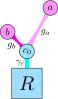
\includegraphics[width=0.3\linewidth, draft=false]{phog/three_mode}
\caption{\label{fig:phog_three_mode} Three-mode model of PhoG device. Two bosonic modes, $a$ and $b$, are each coupled to a third mode, $c_0$. Mode $c_0$ is then strongly coupled to Markovian reservoir $R$ via linear loss $\left(\hat{A} = \hat{a}\right)$ with decay rate $\gamma_c$. }
\end{figure}

The Lindblad equation describing this three-mode model is
\begin{equation}\label{eqn:phog_lindblad_three_mode_model}
\ddt \rho_3 = - i \left[ \hat{H}_3, \rho_3\right] + \left[ \gamma_L \mathcal{L}\left(\hat{a}\right) + \gamma_L \mathcal{L}\left(\hat{b}\right) + \gamma_c \mathcal{L}\left(\hat{c}_0\right)\right] \rho_3
\end{equation}
where the subscript $3$ denotes that we are dealing with this three-mode model. We have taken modes $a$ and $b$ to be coupled to independent Markovian reservoirs with rate $\gamma_L$ which models the conventional linear loss. The Hamiltonian is taken to be $\hat{H}_3 = \hat{H}_3^{\text{int}} + \hat{H}_3^{\text{Kerr}}$, where
\begin{align}\label{eqn:phog_three_mode_hamiltonian}
\hat{H}_3^{\text{int}} &= g_a \hat{a}^\dagger \hat{c}_0 + g_b \hat{b}^\dagger \hat{c}_0 + \hc \notag \\
%
\hat{H}_3^{\text{Kerr}} &= \frac{U}{2} \sum_{x} \hat{x}^\dagger \hat{x}^\dagger \hat{x} \hat{x} \qq{with} \hat{x} \in \left\{\hat{a}, \hat{b}, \hat{c}_0\right\}.
\end{align}
The interaction Hamiltonian $\hat{H}_3^{\text{int}}$ describes linear coupling between modes, while the Kerr Hamiltonian $\hat{H}_3^{\text{Kerr}}$ describes the self-Kerr interaction (self-phase modulation)% Check that these are indeed equivalent
on each mode. This Hamiltonian may be realised, for example, by evanescently coupled waveguides in a $\chi^{\left(3\right)}$ glass. The $U$ is the Kerr nonlinear interaction constant, and we will relate this to glass properties in Sec.~\MT{X} below.

The three-mode model Eq.~\ref{eqn:phog_lindblad_three_mode_model}, while a physically useful starting point for building a system which accurately simulates NCL, is as yet too complicated to difficult to analyse, either analytically or using the numerical methods which proved useful for the single mode model in Secs.~\ref{sec:phog_single_mode_model},~\ref{sec:phog_including_loss}. \MT{I should have an appendix where I discuss the numerical methods which I used in that section.}

We may reduce the complexity of Eq.~\ref{eqn:phog_lindblad_three_mode_model} by assuming that the decay rate $\gamma_c$ of mode $c_0$ into the reservoir $R$ is large enough that mode $c_0$ completely decays on a much faster timescale than modes $a, b$. This will allow for adiabatic elimination of mode $c_0$ via the methods described in Appendix.~\ref{appendix:adiabatic_elimination}. We identify
\begin{align}
H^{\left(0, 0\right)} &= \frac{U}{2} \sum_{x \in \left\{a, b\right\}} x^{\dagger 2} x^2 \notag \\
%
H^{\left(0, 1\right)} &= g_a a^\dagger c_0 + g_b b^\dagger c_0 \notag \\
%
H^{\left(0, 2\right)} = 0
\end{align}
and so, substituting into Eq.~\ref{eqn:adiabatic_elimination}, we arrive at
\begin{equation}\label{eqn:phog_two_mode_model_deriv}
\ddt \rho_2 = - i \left[\frac{U}{2} \sum_{x \in \left\{a, b\right\}} x^{\dagger 2} x^2, \rho_2\right] + \frac{4 G^2}{\gamma_c} \mathcal{L}\left(\frac{g_a a + g_b b}{G} \right)\rho_2 + \gamma_L \left(\mathcal{L}\left(a\right) + \mathcal{L}\left(b\right)\right)\rho_2,
\end{equation}
and so we have reduced our three-mode model to a two-mode system involving only modes $a, b$. Introducing the following collective symmetric and antisymmetric modes

\begin{align}\label{eqn:phog_rotation}
\hat{s}_+ &= \frac{1}{G} \left(g_a \hat{a} + g_b \hat{b}\right) \qq{symmetric}  \notag \\
%
\hat{s}_- &= \frac{1}{G} \left(g_a \hat{b} - g_b \hat{a}\right) \qq{antisymmetric}
\end{align}
with $G = \sqrt{ g_a^2 + g_b^2 }$ required to ensure that $\hat{s}_-, \hat{s}_+$ obey the same bosonic commutation relations as $\hat{a}, \hat{b}$. Rewriting Eq.~\ref{eqn:phog_two_mode_model_deriv} in terms of these new modes we arrive at our two-mode model
\begin{equation}\label{eqn:phog_lindblad_two_mode_model}
\ddt \rho_2 = - i \left[ \hat{H}_2, \rho_2 \right] + \left[ \gamma_L \mathcal{L}\left(\hat{s}_-\right) + \left(\Gamma + \gamma_L\right) \mathcal{L}\left(\hat{s}_+\right) \right] \rho_2
\end{equation}
where the subscript $2$ denotes that each quantity is for this two-mode model, and we have defined $\Gamma = 4 G^2 / \gamma_c$. The Hamiltonian $\hat{H}_2$ takes the form $\hat{H}_2 = \hat{H}_2^{\text{self}} + \hat{H}_2^{\text{int}}$, with
\begin{align}
H_2^{\text{self}} = \varsigma_1\left(n_+^2 + n_-^2\right) + \varsigma_2 n_+ n_- + \varsigma_3\left(n_+ + n_-\right) \notag \\
%
H_2^{\text{int}} = \varsigma_4 \left(s_+^\dagger s_-\right)^2 + \varsigma_5 s_+^\dagger s_- \left(n_- - n_+ - 1\right) + \hc
\end{align}
where $n_{\pm} = s_{\pm}^\dagger s_\pm$ and our $\varsigma$ coefficients are
\begin{align}
\varsigma_1 = \frac{U}{2 G^4} \left(g_a^4 + g_b^4\right), \; \varsigma_2 = \frac{4 U}{G^4} \left(g_a g_b\right)^2, \notag \\
%
\varsigma_3 = \frac{\varsigma_2}{4} - \frac{U}{2}, \; \varsigma_4 = \frac{\varsigma_2}{4}, \; \varsigma_5 = \frac{U}{G^4} g_a g_b \left(g_a^2 - g_b^2\right).
\end{align}
Our two-mode model is depicted in Fig.~\ref{fig:phog_two_mode_model} where we see that mode $s_+$ decays into reservoir $R$ with decay rate $\Gamma + \gamma_L$. In the absence of linear loss, $\gamma_L=0$, mode $s_-$ will decay only vicariously through $s_+$, and the coupling between modes is proportional to nonlinearity parameter $U$. In a linear system, $U = 0$, the antisymmetric mode $s_-$ will not decay and so we identify it as the dark mode of the system which is considered e.g. in Ref.~\MT{Twamley paper}.


\begin{figure}[htp]
\centering
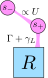
\includegraphics[width=0.3\linewidth, draft=false]{phog/two_mode}
\caption{\label{fig:phog_two_mode_model} Two-mode model of the PhoG device. Having adiabatically eliminated mode $c_0$ from the three-mode model (Fig.~\ref{fig:phog_three_mode}) and rotated to collective basis $s_-, s_+$ using Eqs.~\ref{eqn:phog_rotation} we see that mode $s_-$ will only decay into $R$ by first decaying into $s_+$. The linear coupling between $s_-$ and $s_+$ is proportional to $U$, and so for a linear system $U=0$ mode $s_-$ cannot decay into $R$. $\Gamma = 4 G^2 / \gamma_L$.}
\end{figure}


\MT{Some chat about simulating the two-mode model.}


However, even two bosonic modes are computationally very challenging to simulate when large photon numbers are required \MT{comment about hilbert-space-size-scaling}, and so we seek to adiabatically eliminate mode $s_+$ from the system, which will leave us with an equation for $s_-$ only. 

Let us assume that the decay rate $\Gamma + \gamma_L$ is the dominating decay rate of the two-mode model, and that mode $s_+$ decays to its steady state much quicker than the dynamics of $s_-$. Then applying the adiabatic elimination method described in Appendix~\ref{appendix:adiabatic_elimination} we identify

\begin{align}
H^{\left(0, 0\right)} &= \varsigma_1 n_-^2 + \varsigma_3 n_- \notag \\ 
%
H^{\left(0, 1\right)} &= \varsigma_5 s_-^\dagger n_- \notag \\
%
H^{\left(0, 2\right)} &= \varsigma_4 s_-^{\dagger 2}
\end{align}
and so

\begin{equation}\label{eqn:phog_single_mode_deriv}
\ddt \rho_1 = - i \left[\hat{H}_1, \rho_1\right] + \left\{\gamma_L \mathcal{L}\left(s_-\right) + \gamma_2 \mathcal{L}\left(s_-^2\right) + \gamma_3 \mathcal{L}\left(\ncl\right) \right\}\rho_1
\end{equation}
where we have used the commutator to write $n_- s_- \rightarrow \ncl$, and where
\begin{equation}
\gamma_2 = \frac{4 U^2 \left(g_a g_b\right)^4}{G^8 \left(\Gamma + \gamma_L\right)} \qq{and} \gamma_3 = \frac{4 U^2 \left(g_a g_b\right)^2}{G^8 \left(\Gamma + \gamma_L\right)}\left(g_a^2 - g_b^2\right)^2.
\end{equation}

\noindent We see that Eq.~\ref{eqn:phog_single_mode_deriv} matches Eq.~\ref{eqn:phog_full_single_mode} except for the addition of the Hamiltonian $\hat{H}$ which does not affect the photon-number statistics. 

To summarise, we have reduced the three-mode model (Eq.~\ref{eqn:phog_lindblad_three_mode_model}, Fig.~\ref{fig:phog_three_mode}) to a single-mode model (Eqs.~\ref{eqn:phog_full_single_mode}
,~\ref{eqn:phog_single_mode_deriv}, Fig.~\ref{fig:phog_single_mode}) via two sequential adiabatic eliminations of modes $c_0$ and $s_+$, which rapidly decayed into reservoir $R$. In essence, the behaviour of the antisymmetric collective mode $s_-$ in the three-mode model simulates behaviour of a single mode undergoing both nonlinear coherent loss, two-photon loss and single-photon loss, which were all considered in Secs.~\ref{sec:phog_single_mode_model}~\ref{sec:phog_including_loss}. The combination of Kerr nonlinearity, linear coupling and single-photon loss allows for the effective NCL decay operator to be constructed.

The effective decay rates in this single-mode model explicity depend on coupling constants $g_a, g_b$ (Fig.~\ref{fig:phog_three_mode}, Eq.~\ref{eqn:phog_three_mode_hamiltonian}). We see for example that in the limit of symmetric coupling $g_a = g_b$, $\gamma_3 = 0$ and there will be no NCL for mode $s_-$. Large $\gamma_3$ can be obtained however for strong asymmetry $g_a \gg g_b$ or $g_b \gg g_a$. Since it is NCL which drives $\rho$ most effectively towards highly sub-Poissonian states we will seek to maximise $\gamma_3$.


%\MT{I can't do this until I have motivated the best choice of $g_a, g_b$.}
%We are finally able to give motivation for the choices of $\gamma_2=0.0005, \gamma_3=0.002$ used in Sec.~\ref{sec:phog_summary_ncl_effects} as the 









